\documentclass{article}

\usepackage{graphicx}
\usepackage{tikz}
\usepackage{tikzsymbols}
\usetikzlibrary{calc,patterns,shapes.geometric}
\pagestyle{empty}
\usepackage[margin=0pt]{geometry}
\geometry{papersize={14in,12in}}

\def\centerarc[#1](#2)(#3:#4:#5){\draw[#1] ($(#2)+({#5*cos(#3)},{#5*sin(#3)})$) arc (#3:#4:#5);}

\begin{document}
	\begin{figure}
		\centering
		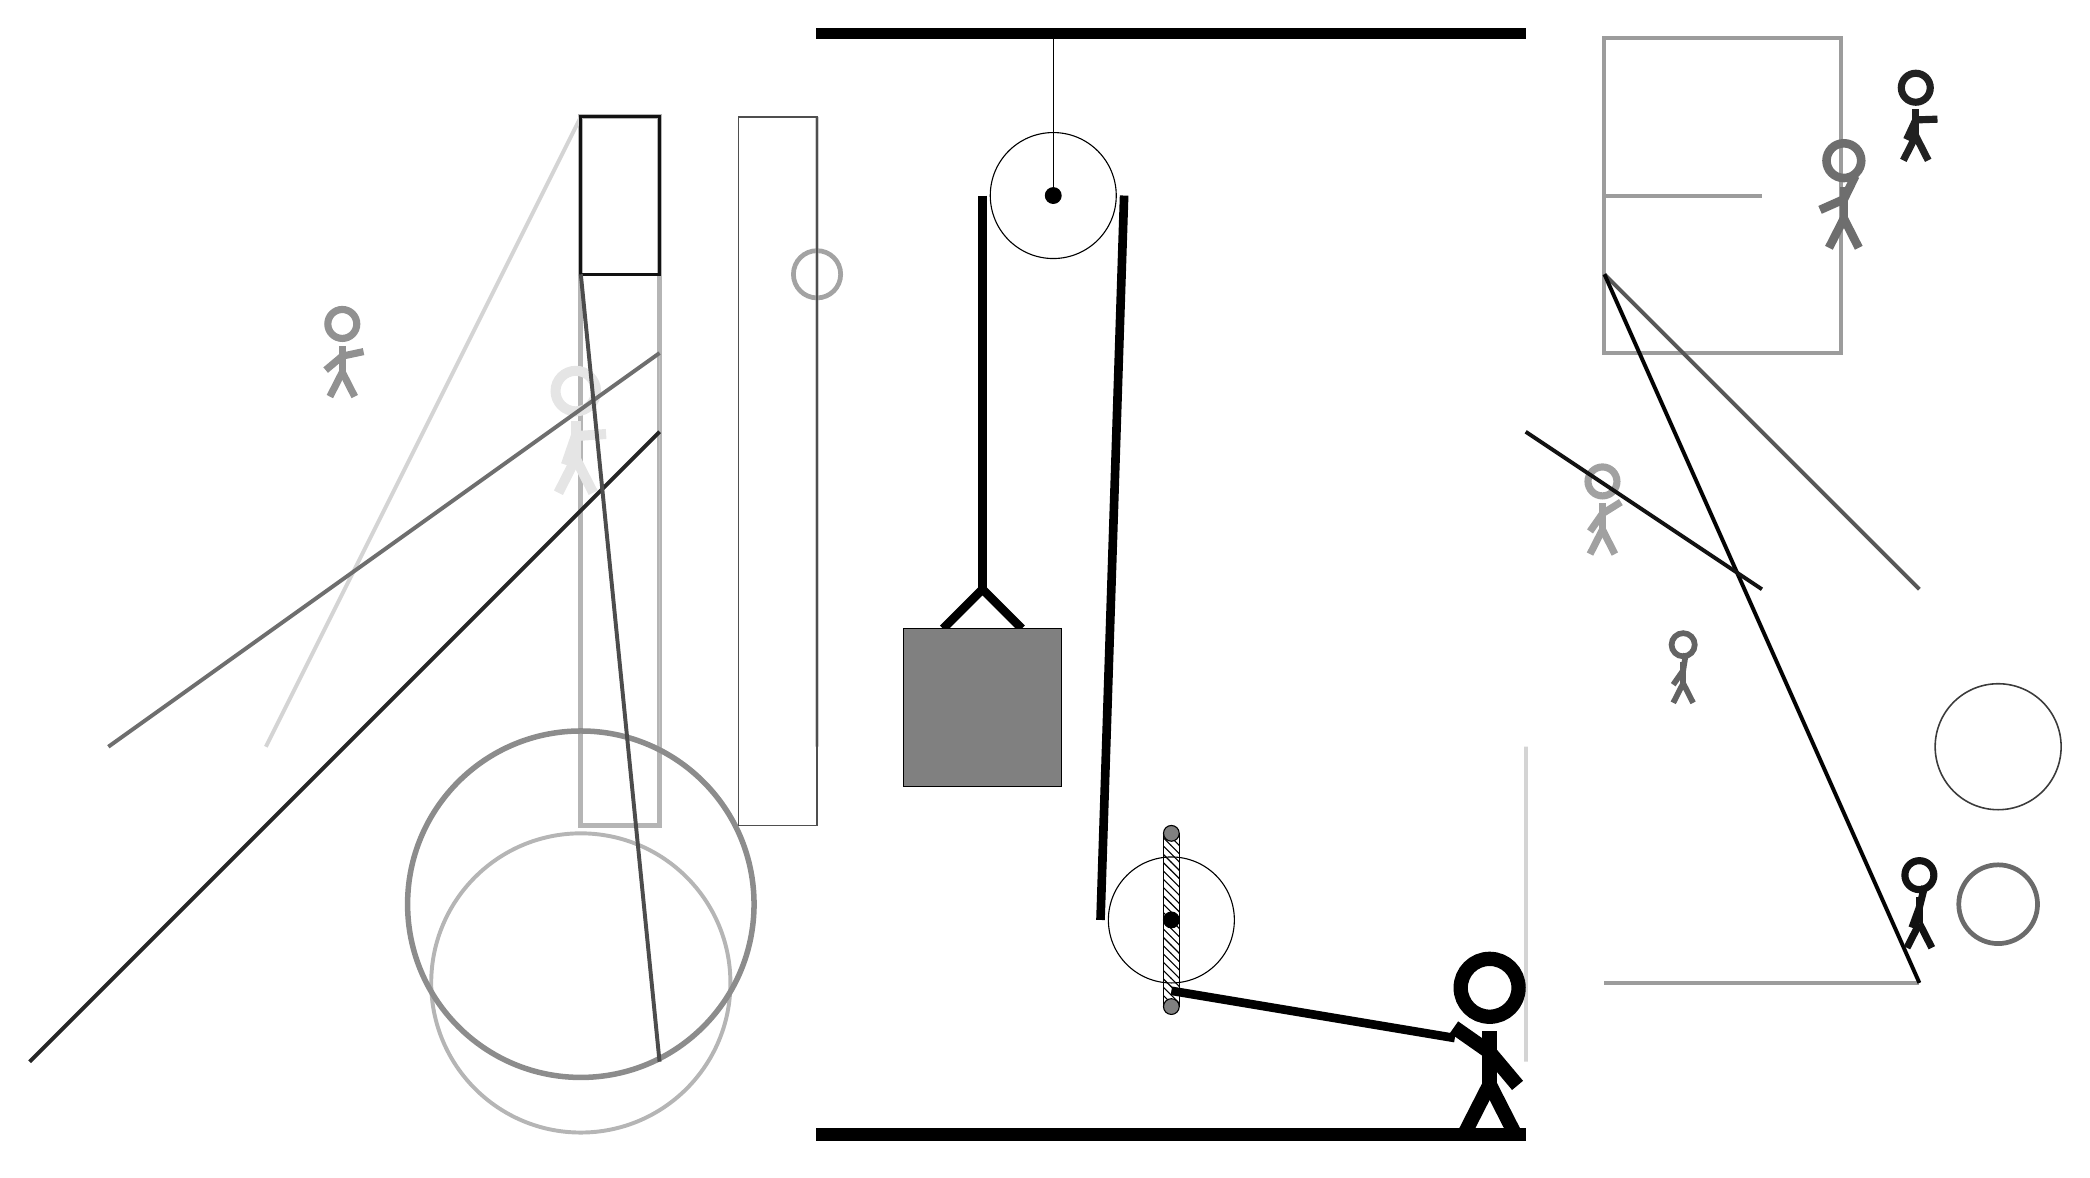
\begin{tikzpicture}
			%%%%% START %%%%%
			
			\draw[fill=black] (-2, 14) rectangle (7, 14.125);
			
			\draw (1, 12) circle (0.8);
			\draw[fill=black] (1, 12) circle (0.1);
			\draw (1, 14) -- (1, 12);
			
			\draw[fill=white](2.5, 2.8) circle (0.8);
			\draw[fill=black] (2.5, 2.8) circle (0.1);
			\draw[pattern=north west lines, pattern color=black] (2.4, 3.9) rectangle (2.6, 1.7);
			\draw[fill=black!50] (2.5, 3.9) circle (0.1);
			\draw[fill=black!50] (2.5, 1.7) circle (0.1);
			
			\draw[line width=1.1mm] (-0.4, 6.5) -- (0.1, 7.0) -- (0.6, 6.5);
			\draw[fill=black!50] (-0.9, 6.5) rectangle (1.1, 4.5);
			
			\draw[line width=0.4mm, color=black!19] (-2, 13) rectangle (-2, 5);
			
			\draw[line width=0.6mm, color=black!29] (-4, 13) rectangle (-5, 4);
			\draw[line width=0.5mm, color=black!39] (8, 10) rectangle (11, 14);
			\node[line width=0.7mm, color=black!37] at (8, 8) {\Strichmaxerl[5][55][32]};
			
			\draw[line width=0.5mm, color=black!17](-5, 13) -- (-9, 5);
			\draw [line width=0.6mm, color=black!58](13, 3) circle (0.5);
			\draw [line width=0.5mm, color=black!29](-5, 2) circle (1.9);
			\draw[line width=0.5mm, color=black!17] (7, 5) rectangle (7, 1);
			\draw[line width=0.5mm, color=black!66](12, 7) -- (8, 11);
			
			\draw [line width=0.2mm, color=black!77](13, 5) circle (0.8);
			\draw[line width=0.2mm, color=black!24] (-4, 5) rectangle (-4, 10);
			
			\node[line width=0.5mm, color=black!10] at (-5, 9) {\Strichmaxerl[7][71][4]};
			\node[line width=0.5mm, color=black!57] at (11, 12) {\Strichmaxerl[6][24][64]};
			
			\draw[line width=0.4mm, color=black!93] (-4, 13) rectangle (-5, 11);
			\draw [line width=0.6mm, color=black!36](-2, 11) circle (0.3);
			\draw[line width=0.5mm, color=black!85](-4, 9) -- (-12, 1);
			
			\node[line width=0.4mm, color=black!61] at (9, 6) {\Strichmaxerl[4][55][81]};
			\node[line width=0.3mm, color=black!87] at (12, 13) {\Strichmaxerl[5][65][2]};
			\draw [line width=0.7mm, color=black!45](-5, 3) circle (2.2);
			\node[line width=0.6mm, color=black!43] at (-8, 10) {\Strichmaxerl[5][40][12]};
			\draw[line width=0.5mm, color=black!39](8, 2) -- (12, 2);
			
			\draw[line width=0.5mm, color=black!39] (8, 12) rectangle (10, 12);
			\draw[line width=0.5mm, color=black!99](12, 2) -- (8, 11);
			\draw[line width=0.5mm, color=black!57](-4, 10) -- (-11, 5);
			\node[line width=0.2mm, color=black!93] at (12, 3) {\Strichmaxerl[5][70][76]};
			
			\draw[line width=0.5mm, color=black!93](7, 9) -- (10, 7);
			\draw[line width=0.5mm, color=black!70](-4, 1) -- (-5, 11);
			\draw [line width=0.5mm, color=black!93](13, 12) circle (0.0);
			\draw[line width=0.2mm, color=black!69] (-2, 4) rectangle (-3, 13);
			
			\draw[line width=1.1mm] (0.1, 12) -- (0.1, 7.0);
			\centerarc[line width=1.1mm](1, 12)(0:180:0.9);
			\draw[line width=1.1mm](1.9, 12) -- (1.6, 2.8);
			\centerarc[line width=1.1mm](2.5, 2.8)(180:270:0.9);
			\draw[line width=1.1mm](2.5, 1.9) -- (6.1, 1.3);
			
			\node at (6.5, 1.2) {\Strichmaxerl[10][-35][-50]};
			
			\draw[fill=black] (-2, 0) rectangle (7, 0.15);
			
			%%%%% END %%%%%
		\end{tikzpicture}
	\end{figure}	
\end{document}